\documentclass[12pt,a4paper]{article}
\usepackage[utf8]{inputenc}
\usepackage{amsmath}
\usepackage[]{units}
\usepackage{breqn}
\usepackage{amsfonts}
\usepackage{amssymb}
\usepackage{graphicx}
\usepackage[margin=0.8in]{geometry}


\begin{document}
\title{\vspace{70mm}\Huge Experimento 02 - Pêndulo de Torção}
\author{ Giovani Garuffi\qquad\hfill
		\textit {RA: 155559}\protect\\
		João Baraldi\hfill
		\textit{RA: 158044}\protect\\
		Lauro Cruz\hfill
		\textit{RA: 156175}\protect\\
		Lucas Schanner\hfill
		\textit{RA: 156412}\protect\\
		Pedro Stringhini\hfill
		\textit {RA: 156983}								
		}
\maketitle
\newpage
\section{Resumo}


\section{Objetivos}


\section{Procedimento Experimental e Coleta de Dados}

\subsection{Materiais utilizados}
\begin{itemize}
	\item Pêndulo de torção com fio metálico
	\item Trena
	\item Paquímetro
	\item Micrômetro
	\item Photo-gate
	\item Cronômetro inteligente
\end{itemize}

\subsection{Procedimento}
O pêndulo foi montado usando-se um fio metálico tendo um cilindro de latão acoplado em sua ponta. Foram medidos o diâmetro do fio (com o micrômetro) e contabilizada a massa do cilindro (já previamente neles explicitada). Ao lado do da base do pêndulo, foi montado o photo-gate conectado a um cronômetro inteligente configurado no modo \emph{Pendulum}, para ser realizada a medição dos perídos de rotação. Para cada comprimento L do fio foram feitas 7 medições de período para fazer-se assim uma média aritmética. Todas as medições mencionadas foram registradas no relatório. 

\begin{figure}[!htbp]
	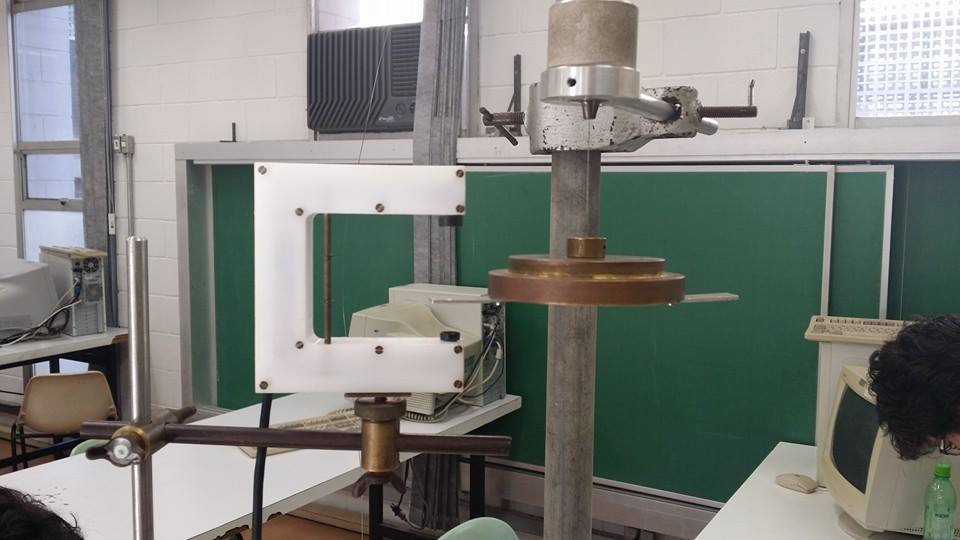
\includegraphics[scale=0.50]{03.jpg}
	\caption{Medição dos períodos}
	\label{fig:cilindro}
\end{figure}

\begin{figure}[!htbp]
	\centering
	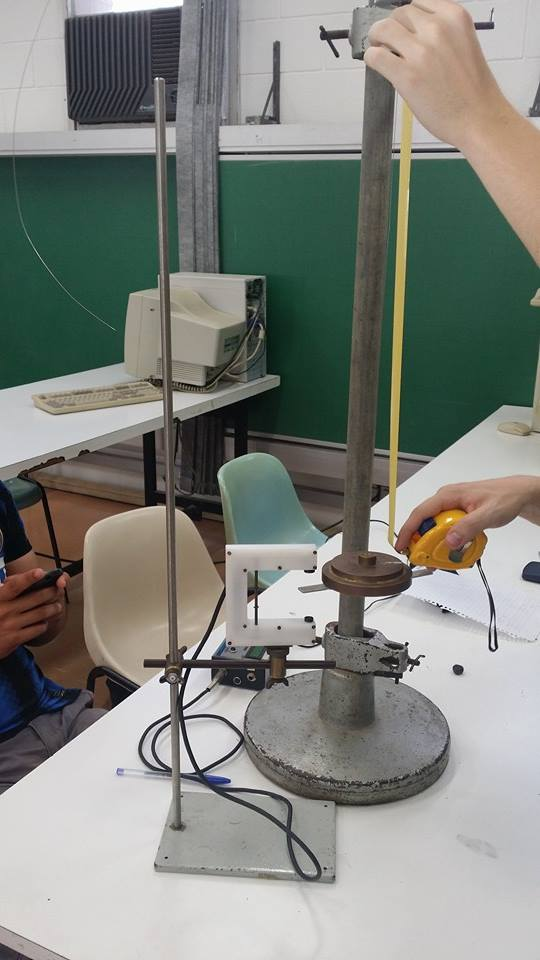
\includegraphics[scale=0.30]{01.jpg}
	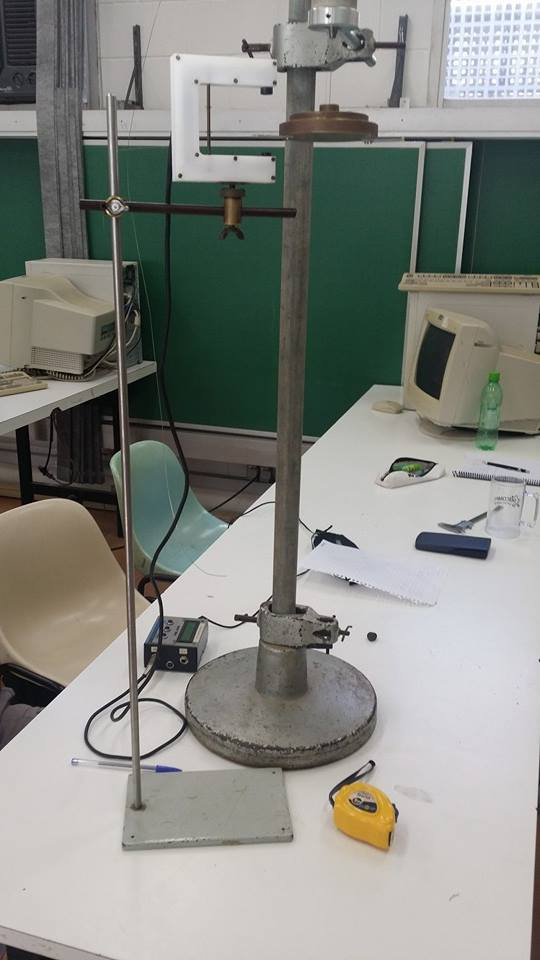
\includegraphics[scale=0.30]{02.jpg}\\
	Figures 1, 2: Montagem
\end{figure}

\subsection{Dados Obtidos}
O valor do diâmetro do fio é:
$$ d = (0.56 \pm 0.01) mm, $$
sendo $0.01 mm$ o erro intrumental do micrômetro.\\\\
A massa do conjunto de cilindros, previamente medida, é:
$$ M = (1198.2 \pm 0.1) g,$$
sendo $0.1 g$ o erro intrumental da balança usada.\\\\
Os valores dos períodos medidos (T) para cada comprimento da linha (L): % Aqui vai ser colocado a tabela, confere?

\subsubsection{Analise do cilindro}
Para fazer o cálculo do momento de inércia do cilindro utilizado no pêndulo ele foi subdividido em três cilindros (Figure \ref{fig:cilindro}), e foram medidos os diâmetros e alturas de cada um, para assim calcular seus volumes e determinar a massa de cada um separadamente.

Diâmetros:
$$ D_1 = (20.05 \pm 0.05)mm, $$
$$ D_2 = (80.15 \pm 0.05)mm, $$
$$ D_3 = (99.35 \pm 0.05)mm, $$

e Alturas:
$$ h_1 = (10.05 \pm 0.05)mm, $$
$$ h_2 = (8.05 \pm 0.05)mm, $$
$$ h_3 = (12.40 \pm 0.05)mm, $$

sendo $0.05mm$ o erro instrumental do paquímetro.\\

A partir de suas dimensões, o volume ($V_n$) e seu erro ($\Delta V_n$) de cada cilindro foi calculado a partir da fórmula
$$V_n = \frac{\pi D_n^2 h_n}{4}, \; \; \;  \; \Delta V_n = \frac {\pi D_n^2}{4} \sqrt{h_n^2 \Delta r_n^2 + r^2 \Delta h_n^2},$$
resultando em:
$$V_2 = , \; \; \; \; \Delta V_1 = ,$$
$$V_2 = , \; \; \; \; \Delta V_2 = ,$$ 
$$V_3 = , \; \; \; \; \Delta V_3 = .$$ 

Desse modo, e considerando as massas dos cilindros praticamente homogêneas, foi determinado a massa de cada um em relação ao total $M$ a a partir da relação
$$M_n = \frac{V_n}{V} M, \; \; \; \; \Delta M_n = \sqrt{\frac{M^2}{V^2} \Delta V_n^2 + \frac{V_n^2}{V^2} \Delta M^2 + \frac{V_n^2}{V^4} \Delta V^2},$$
sendo $V$ o volume total dos cilindros e $\Delta V = \sqrt{3} \Delta V_cilindro$, levando em conta que os erros do volume dos cilindros é cte.
Com isso, tem-se que:
$$M_1 = , \; \; \; \; \Delta M_1 = ,$$
$$M_2 = , \; \; \; \; \Delta M_2 = ,$$
$$M_3 = , \; \; \; \; \Delta M_3 = .$$

Calcula-se, a partir daí, o Momento de inércia $I_{0n}$ de cada cilindro com seu erro $\Delta I_{0n}$. Sabendo que:
$$I_{0n} = \frac{M_nD_n^2}{8}, \; \; \; \; \Delta I_{0n} = \frac {1}{2} \sqrt{M_n^2D_n^2 \Delta D_n^2 + \frac{D_n^2}{4} \Delta M_n^2},$$

Então,
$$I_{01} =, \; \; \; \; \Delta I_{01} = ,$$
$$I_{02} =, \; \; \; \; \Delta I_{02} = ,$$
$$I_{03} =, \; \; \; \; \Delta I_{03} = ,$$
e logo, como o momento de inércia total $I_0$ é a soma dos momentos de inércia dos cilindros,
$$I_0 = , \; \; \; \; \Delta I_0 = .$$.
\section{Análise dos Resultados e Discussões}



\subsection{Determinação do módulo de cisalhamento}
%Determinação da reta e explicação dos coeficientes aqui, e depois... %
O módulo de cisalhamento $G$ do material do fio e seu erro podem ser expressos, em função do coeficiente angular da reta, por meio da relação
$$G = 8\pi\frac {I_0}{ar^4}, \; \; \; \; \Delta G = \frac {8\pi}{ar^4} \sqrt{\Delta I_0^2 + I_0^2 \Delta a^2 + 16 \frac{I_0^2}{r^{10}} \Delta r^2}.$$

\section{Conclusões}


\end{document}
